% Options for packages loaded elsewhere
\PassOptionsToPackage{unicode}{hyperref}
\PassOptionsToPackage{hyphens}{url}
%
\documentclass[
]{article}
\usepackage{amsmath,amssymb}
\usepackage{iftex}
\ifPDFTeX
  \usepackage[T1]{fontenc}
  \usepackage[utf8]{inputenc}
  \usepackage{textcomp} % provide euro and other symbols
\else % if luatex or xetex
  \usepackage{unicode-math} % this also loads fontspec
  \defaultfontfeatures{Scale=MatchLowercase}
  \defaultfontfeatures[\rmfamily]{Ligatures=TeX,Scale=1}
\fi
\usepackage{lmodern}
\ifPDFTeX\else
  % xetex/luatex font selection
\fi
% Use upquote if available, for straight quotes in verbatim environments
\IfFileExists{upquote.sty}{\usepackage{upquote}}{}
\IfFileExists{microtype.sty}{% use microtype if available
  \usepackage[]{microtype}
  \UseMicrotypeSet[protrusion]{basicmath} % disable protrusion for tt fonts
}{}
\makeatletter
\@ifundefined{KOMAClassName}{% if non-KOMA class
  \IfFileExists{parskip.sty}{%
    \usepackage{parskip}
  }{% else
    \setlength{\parindent}{0pt}
    \setlength{\parskip}{6pt plus 2pt minus 1pt}}
}{% if KOMA class
  \KOMAoptions{parskip=half}}
\makeatother
\usepackage{xcolor}
\usepackage[margin=1in]{geometry}
\usepackage{longtable,booktabs,array}
\usepackage{calc} % for calculating minipage widths
% Correct order of tables after \paragraph or \subparagraph
\usepackage{etoolbox}
\makeatletter
\patchcmd\longtable{\par}{\if@noskipsec\mbox{}\fi\par}{}{}
\makeatother
% Allow footnotes in longtable head/foot
\IfFileExists{footnotehyper.sty}{\usepackage{footnotehyper}}{\usepackage{footnote}}
\makesavenoteenv{longtable}
\usepackage{graphicx}
\makeatletter
\def\maxwidth{\ifdim\Gin@nat@width>\linewidth\linewidth\else\Gin@nat@width\fi}
\def\maxheight{\ifdim\Gin@nat@height>\textheight\textheight\else\Gin@nat@height\fi}
\makeatother
% Scale images if necessary, so that they will not overflow the page
% margins by default, and it is still possible to overwrite the defaults
% using explicit options in \includegraphics[width, height, ...]{}
\setkeys{Gin}{width=\maxwidth,height=\maxheight,keepaspectratio}
% Set default figure placement to htbp
\makeatletter
\def\fps@figure{htbp}
\makeatother
\setlength{\emergencystretch}{3em} % prevent overfull lines
\providecommand{\tightlist}{%
  \setlength{\itemsep}{0pt}\setlength{\parskip}{0pt}}
\setcounter{secnumdepth}{5}
\usepackage[french]{babel}
\usepackage[utf8]{inputenc}
\usepackage{geometry}
\geometry{margin=2.5cm}
\usepackage{float}
\usepackage{graphicx}
\renewcommand{\contentsname}{Sommaire}
\ifLuaTeX
  \usepackage{selnolig}  % disable illegal ligatures
\fi
\usepackage{bookmark}
\IfFileExists{xurl.sty}{\usepackage{xurl}}{} % add URL line breaks if available
\urlstyle{same}
\hypersetup{
  pdftitle={Projet TND - Analyse des céréales},
  pdfauthor={Trinome 5},
  hidelinks,
  pdfcreator={LaTeX via pandoc}}

\title{Projet TND - Analyse des céréales}
\author{Trinome 5}
\date{2025-2026}

\begin{document}
\maketitle

{
\setcounter{tocdepth}{2}
\tableofcontents
}
\listoffigures

\section{Introduction}\label{introduction}

Ce rapport porte sur 77 céréales de petit-déjeuner vendues aux
États-Unis. On cherche à voir comment elles se distinguent sur le plan
nutritionnel, et s'il existe des groupes de céréales qui se ressemblent.

Chaque céréale est décrite par 16 variables : des données
nutritionnelles (calories, protéines, graisses, etc.), des informations
de conditionnement (poids, taille de portion) et quelques métadonnées
(fabricant, type de consommation, note de satisfaction). Les unités sont
très hétérogènes : des Kcal, des grammes, des milligrammes, une note sur
100. C'est ce qui nous a poussés vers une ACP normée plutôt qu'une ACP
classique.

On a donc commencé par une ACP normée pour résumer l'information et
regarder comment les variables sont reliées, puis on a appliqué deux
méthodes de classification, la CAH et les K-means, pour voir si des
profils nutritionnels se dégagent.

\section{Description des données}\label{description-des-donnuxe9es}

\subsection{Présentation du jeu de
données}\label{presentation-du-jeu-de-donnuxe9es}

Le fichier \texttt{276-cereals.txt} contient 77 céréales et 16
variables. En regardant la structure, on retrouve trois types de
variables :

\begin{itemize}
\tightlist
\item
  \textbf{Identifiant} : NAME (nom de la céréale)
\item
  \textbf{Variables qualitatives} : MANUF (fabricant, 7 modalités : A,
  G, K, N, P, Q, R) et TYPE (C = consommation froide, H = chaude)
\item
  \textbf{Variables quantitatives} (13) : CALORIES, PROTEIN, FAT,
  SODIUM, FIBER, CARBO, SUGARS, POTASS, VITAMINS, SHELF, WEIGHT, CUPS,
  RATING
\end{itemize}

La répartition est déséquilibrée : 74 céréales froides pour seulement 3
chaudes. Côté fabricants, Kellogg's (K, 23 céréales) et General Mills
(G, 22) représentent à eux deux plus de la moitié du jeu de données.

\subsection{Prétraitement}\label{pretraitement}

Certaines valeurs valent -1 dans le fichier d'origine. Une valeur
négative n'ayant aucun sens pour un contenu nutritionnel, on les a
traitées comme des données manquantes. Il y en a 4 au total : 2 sur
POTASS, 1 sur CARBO, 1 sur SUGARS.

On les a remplacées par la médiane de chaque variable. La médiane
résiste mieux que la moyenne aux valeurs extrêmes, ce qui compte ici
parce que des variables comme FIBER ou POTASS ont des distributions très
étalées.

\subsection{Définition des rôles pour
l'ACP}\label{duxe9finition-des-roles-pour-lacp}

Pour l'ACP, on a gardé 9 variables actives, celles qui décrivent
vraiment la composition nutritionnelle : CALORIES, PROTEIN, FAT, SODIUM,
FIBER, CARBO, SUGARS, POTASS et VITAMINS.

SHELF, WEIGHT, CUPS et RATING passent en variables supplémentaires
quantitatives : elles n'entrent pas dans le calcul des axes mais on les
projette ensuite pour aider à l'interprétation. MANUF et TYPE sont des
variables supplémentaires qualitatives.

Ce découpage se justifie facilement : WEIGHT et CUPS parlent du
conditionnement, pas du contenu. RATING est une note calculée par
Consumer Reports ; comme c'est une variable construite à partir des
autres, on préfère la regarder à part pour voir où elle tombe par
rapport aux axes nutritionnels.

\section{Statistiques descriptives}\label{statistiques-descriptives}

\subsection{Analyse univariée}\label{analyse-univariuxe9e}

Le tableau ci-dessous reprend les principales statistiques des variables
actives :

\begin{longtable}[]{@{}lrrrr@{}}
\caption{Statistiques des variables actives}\tabularnewline
\toprule\noalign{}
& Moyenne & Médiane & Écart-type & Skewness \\
\midrule\noalign{}
\endfirsthead
\toprule\noalign{}
& Moyenne & Médiane & Écart-type & Skewness \\
\midrule\noalign{}
\endhead
\bottomrule\noalign{}
\endlastfoot
CALORIES & 106.9 & 110.0 & 19.5 & -0.44 \\
PROTEIN & 2.5 & 3.0 & 1.1 & 0.73 \\
FAT & 1.0 & 1.0 & 1.0 & 1.14 \\
SODIUM & 159.7 & 180.0 & 83.8 & -0.56 \\
FIBER & 2.2 & 2.0 & 2.4 & 2.38 \\
CARBO & 14.8 & 14.5 & 3.9 & 0.11 \\
SUGARS & 7.0 & 7.0 & 4.3 & 0.04 \\
POTASS & 98.4 & 90.0 & 69.5 & 1.40 \\
VITAMINS & 28.2 & 25.0 & 22.3 & 2.42 \\
\end{longtable}

Deux ou trois choses ressortent. FIBER (skewness = 2.38) et VITAMINS
(2.42) sont fortement étalées vers la droite : la plupart des céréales
en contiennent peu, sauf quelques cas extrêmes. SUGARS, au contraire,
est presque symétrique (skewness = 0.04) ; les céréales se répartissent
à peu près également entre peu et très sucrées.

\begin{figure}[H]

{\centering 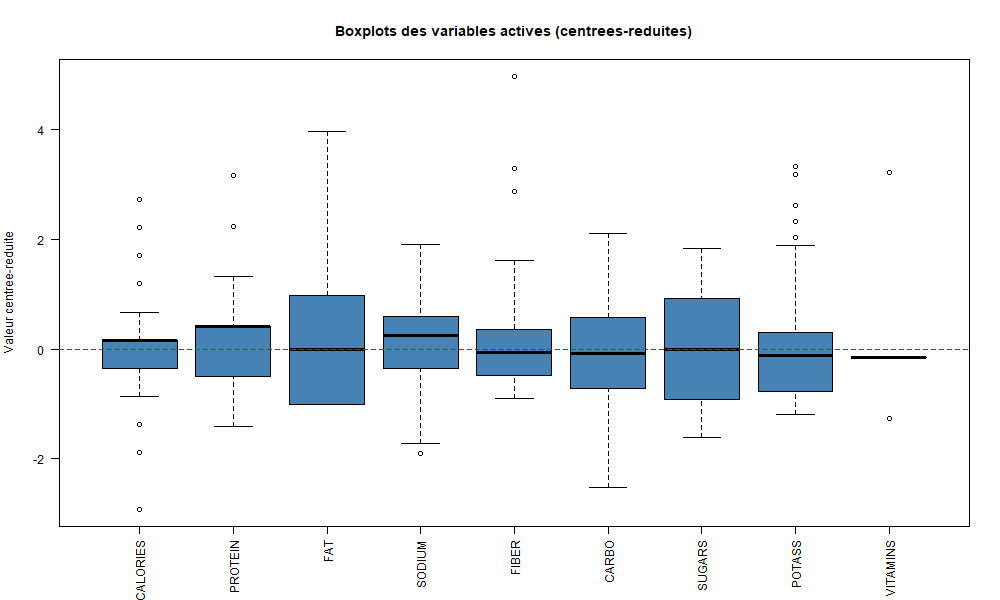
\includegraphics[width=0.9\linewidth]{output/figures/01_boxplots_actives} 

}

\caption{Boxplots des variables actives (centrées-réduites)}\label{fig:boxplots}
\end{figure}

Les boxplots font apparaître plusieurs valeurs atypiques, surtout sur
FIBER et POTASS (les All-Bran) et sur VITAMINS (les ``Total'' enrichies
à 100\% des apports). On a choisi de les garder : ce sont de vraies
céréales du marché, même si elles sortent du lot.

\subsection{Analyse bivariée}\label{analyse-bivariuxe9e}

\begin{figure}[H]

{\centering 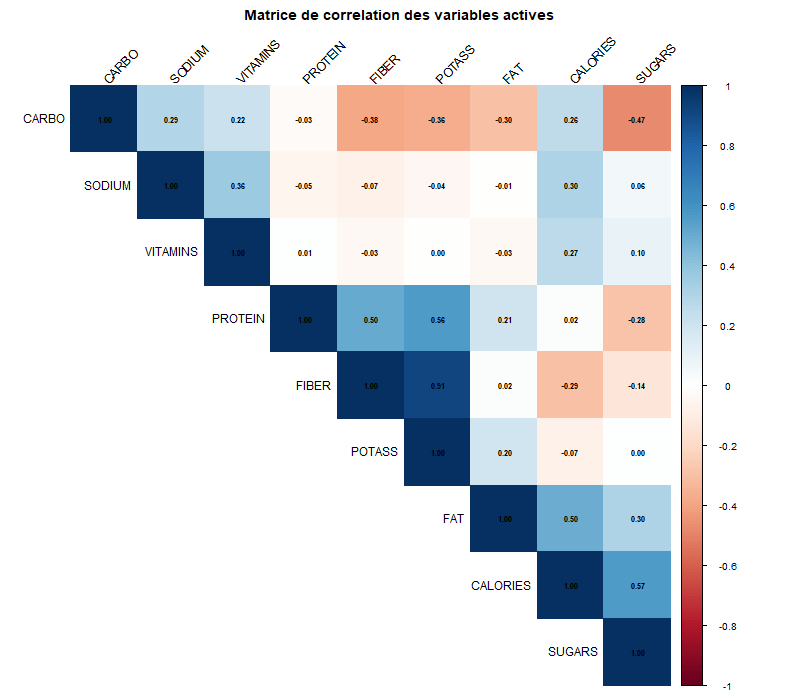
\includegraphics[width=0.8\linewidth]{output/figures/03_heatmap_correlation} 

}

\caption{Matrice de corrélation des variables actives}\label{fig:heatmap}
\end{figure}

La matrice de corrélation est plutôt parlante. La corrélation la plus
forte relie FIBER et POTASS (r = 0.91), ce qui se comprend bien : les
céréales complètes, riches en fibres, gardent les minéraux du grain,
dont le potassium. CALORIES est aussi corrélé à SUGARS (r = 0.57) et à
FAT (r = 0.50) : sans surprise, sucres et graisses apportent des
calories.

CARBO est corrélé négativement à SUGARS (r = -0.47). Ça paraît étrange
au premier abord, mais en pratique les céréales riches en glucides
complexes (amidon) sont souvent peu sucrées : le sucre remplace l'amidon
au lieu de s'y ajouter.

Ces corrélations expliquent pourquoi une ACP a du sens ici : les 9
variables sont loin d'être indépendantes, et réduire la dimension permet
de mieux voir leur structure.

\section{Analyse en composantes
principales}\label{analyse-en-composantes-principales}

\subsection{Choix de l'ACP normée}\label{choix-de-lacp-normuxe9e}

Comme les variables sont dans des unités différentes (Kcal, grammes,
milligrammes, note), une ACP non normée donnerait beaucoup trop de poids
aux variables à forte variance comme SODIUM (écart-type = 84) ou POTASS
(écart-type = 69) face à FAT (écart-type = 1). L'ACP normée travaille
sur la matrice de corrélation, après centrage-réduction, et met donc
toutes les variables sur un pied d'égalité.

\subsection{Valeurs propres et nombre
d'axes}\label{valeurs-propres-et-nombre-daxes}

\begin{figure}[H]

{\centering 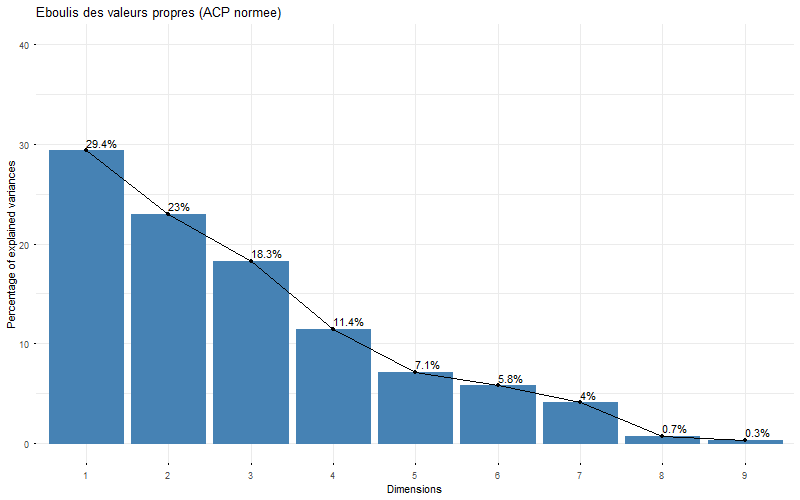
\includegraphics[width=0.75\linewidth]{output/figures/06_scree_plot} 

}

\caption{Éboulis des valeurs propres}\label{fig:scree}
\end{figure}

Le critère de Kaiser (valeurs propres \textgreater{} 1) retient 4 axes,
qui couvrent 82.1\% de l'inertie. Les deux premiers en cumulent déjà
52.4\%, ce qui reste correct pour 9 variables. Le scree plot ne montre
pas de coude franc, plutôt une décroissance régulière. On fera
l'essentiel des interprétations sur le plan (1,2), en gardant en tête
que les axes 3 et 4 portent encore une part non négligeable de
l'information.

\subsection{Cercle des corrélations}\label{cercle-des-corruxe9lations}

\begin{figure}[H]

{\centering 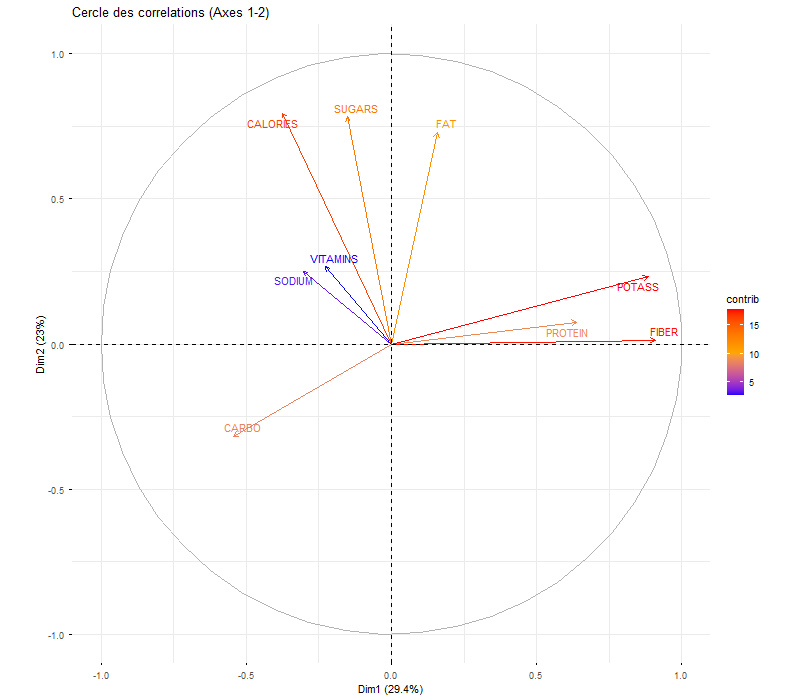
\includegraphics[width=0.7\linewidth]{output/figures/07_cercle_correlations_12} 

}

\caption{Cercle des corrélations (axes 1-2)}\label{fig:cercle}
\end{figure}

L'axe 1 (29.4\% d'inertie) est surtout tiré par FIBER et POTASS du côté
positif. On peut le lire comme un gradient de richesse en fibres : à
droite les céréales riches en fibres et en potassium, à gauche celles
qui en sont pauvres.

L'axe 2 (23.0\%) oppose CALORIES, FAT et SUGARS (en haut) à un pôle plus
neutre (en bas). C'est l'axe de la densité calorique : en haut, les
céréales les plus caloriques, les plus grasses et les plus sucrées.

SODIUM et VITAMINS sont mal représentés sur ce plan (vecteurs courts),
ce qui confirme qu'ils sont surtout portés par les axes 3 et 4. CARBO se
retrouve dans le cadran bas-gauche, à l'opposé de SUGARS : on retrouve
l'opposition glucides complexes / sucres simples déjà vue dans les
corrélations.

\subsection{Carte des individus et
biplot}\label{carte-des-individus-et-biplot}

\begin{figure}[H]

{\centering 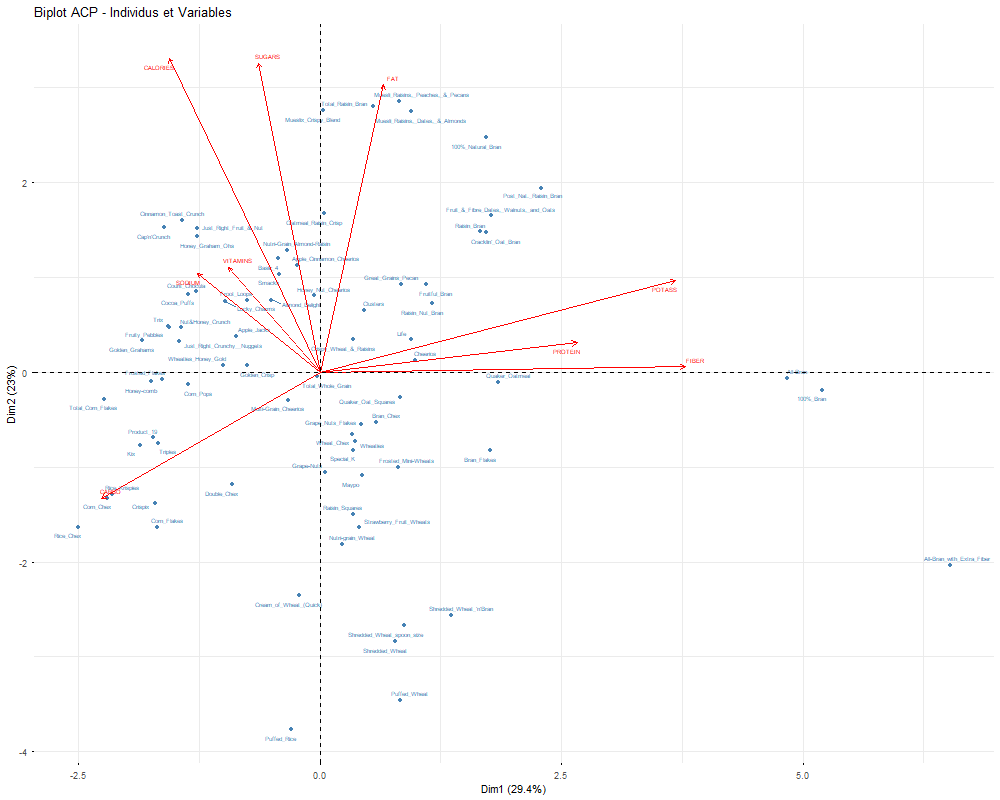
\includegraphics[width=0.85\linewidth]{output/figures/10_biplot} 

}

\caption{Biplot - individus et variables}\label{fig:biplot}
\end{figure}

Le biplot permet de regarder céréales et variables en même temps. Les
trois All-Bran (100\% Bran, All-Bran, All-Bran with Extra Fiber) se
détachent nettement à droite, du côté des fibres. À l'opposé, on trouve
Rice Chex, Corn Chex et les autres céréales à base de riz ou de maïs,
pauvres en fibres.

En haut, les céréales sucrées (Cap'n'Crunch, Froot Loops, Lucky Charms)
suivent les vecteurs SUGARS et CALORIES. En bas, les céréales peu
caloriques type Puffed Rice ou Shredded Wheat.

\subsection{Variables
supplémentaires}\label{variables-suppluxe9mentaires}

RATING se projette avec une coordonnée positive sur l'axe 1 (+0.62) et
négative sur l'axe 2 (-0.72). Autrement dit, les céréales bien notées
par Consumer Reports sont riches en fibres et pauvres en calories et en
sucres. La note suit donc d'assez près la qualité nutritionnelle telle
que la décrivent les axes de l'ACP.

Pour les fabricants, Nabisco (N) se place clairement dans le coin fibres
élevées / peu calorique, ce qui colle avec sa gamme Shredded Wheat.
General Mills (G) et Kellogg's (K) restent plus au centre, avec des
gammes variées. Les 3 céréales chaudes (H) se projettent à part des
froides, mais elles sont trop peu nombreuses pour en conclure quoi que
ce soit.

\section{Classification}\label{classification}

\subsection{CAH - Méthode de Ward}\label{cah---methode-de-ward}

\begin{figure}[H]

{\centering 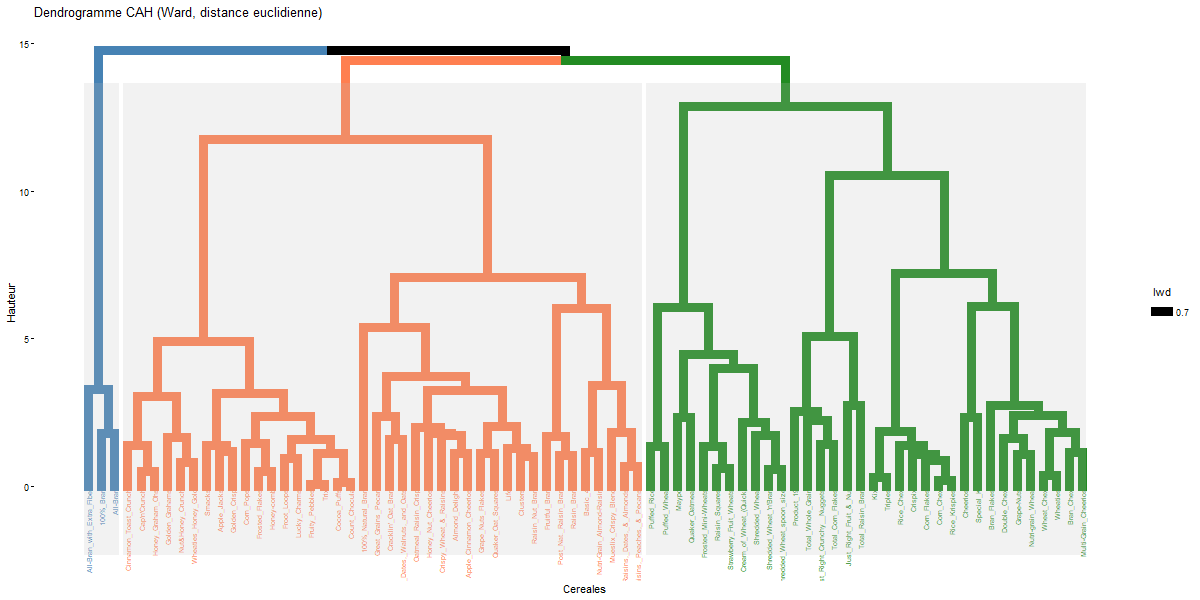
\includegraphics[width=0.95\linewidth]{output/figures/12_dendrogramme} 

}

\caption{Dendrogramme (CAH, Ward, distance euclidienne)}\label{fig:dendrogramme}
\end{figure}

On lance la CAH avec la distance euclidienne sur les données
centrées-réduites et le critère de Ward, qui minimise la hausse
d'inertie intra-classe à chaque fusion. Ce critère va bien avec la
distance euclidienne et donne en général des classes de tailles proches.

Le dendrogramme penche pour une partition en 3 classes, avec un saut
d'inertie net entre 3 et 2 clusters. La silhouette moyenne à k=3 vaut
0.21, ce qui est faible. À k=2 elle monte à 0.45, donc plus propre, mais
on perd alors le groupe des céréales très riches en fibres, qui nous
intéresse.

\begin{figure}[H]

{\centering 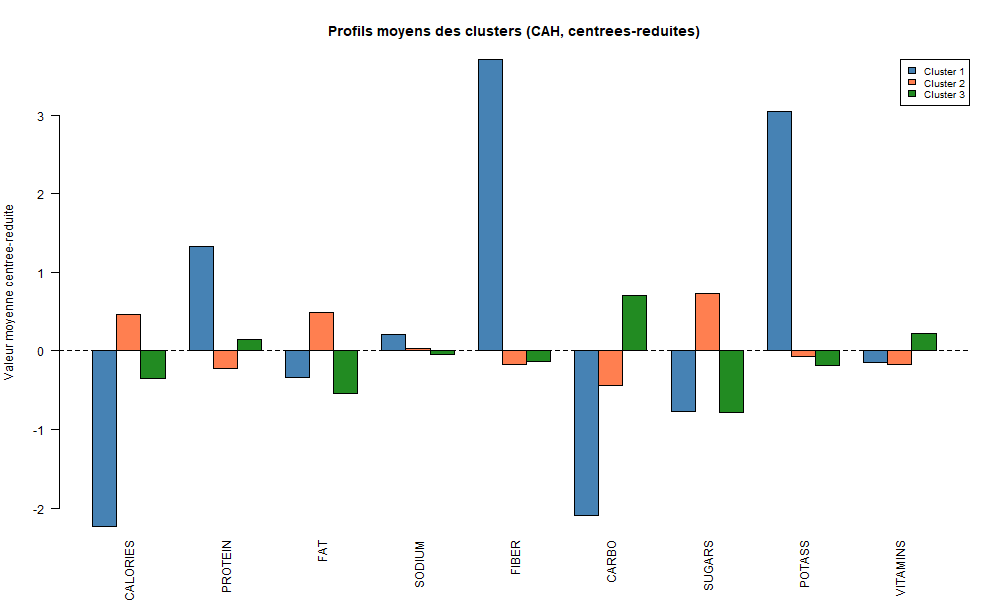
\includegraphics[width=0.7\linewidth]{output/figures/14_profils_cah} 

}

\caption{Profils moyens des 3 clusters (CAH, données centrées-réduites)}\label{fig:profils-cah}
\end{figure}

Les trois clusters obtenus sont :

\begin{itemize}
\tightlist
\item
  \textbf{Cluster 1} (3 céréales) : profil ``haute fibre''. FIBER et
  POTASS très élevés, CALORIES et CARBO faibles. Ce sont les trois
  céréales All-Bran.
\item
  \textbf{Cluster 2} (40 céréales) : profil ``sucre/calorique''. SUGARS
  et CALORIES au-dessus de la moyenne, FIBER et CARBO en dessous.
\item
  \textbf{Cluster 3} (34 céréales) : profil ``modéré''. Peu de sucre,
  peu de gras, CARBO élevé. Ce sont des céréales de type classique (Corn
  Flakes, Rice Krispies, etc.).
\end{itemize}

Le cluster 1 ne compte que 3 individus, ce qui le rend fragile. Ce sont
en réalité des outliers nutritionnels plus qu'un vrai ``type''
commercial de céréale. Cela dit, leur séparation est franche et
reproductible.

\subsection{K-means}\label{k-means}

On refait une classification en K-means avec le même k=3 pour comparer.
On met nstart=25 pour limiter l'effet du tirage initial, l'algorithme
n'étant pas déterministe contrairement à la CAH.

\begin{figure}[H]

{\centering 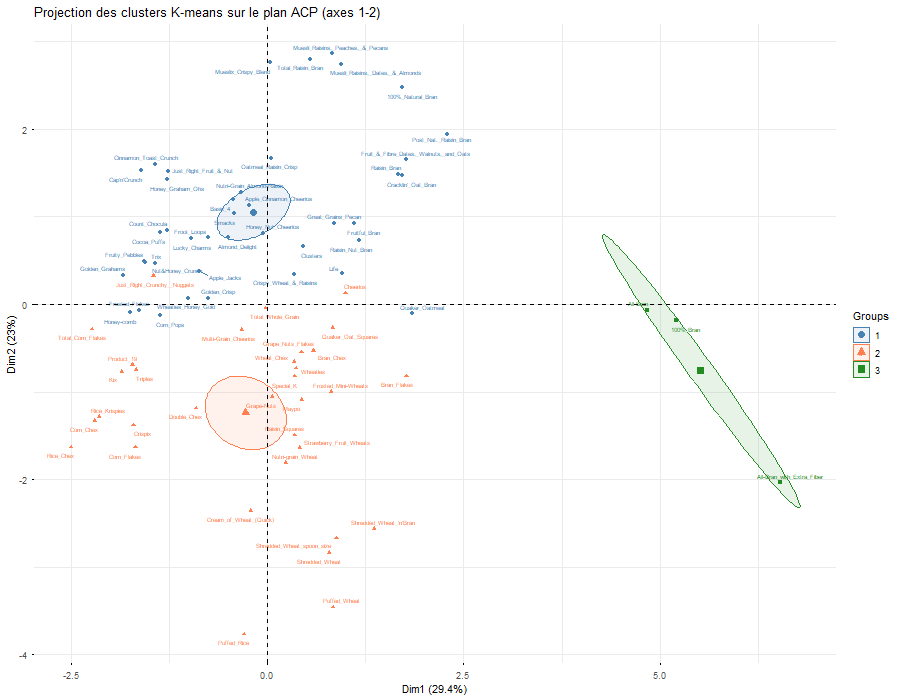
\includegraphics[width=0.8\linewidth]{output/figures/19_acp_clusters_kmeans} 

}

\caption{Projection des clusters K-means sur le plan ACP}\label{fig:clusters-acp}
\end{figure}

Les clusters K-means ressemblent beaucoup à ceux de la CAH. Sur le plan
ACP, la séparation est nette : le groupe ``haute fibre'' est isolé à
droite, le groupe ``sucre'' en haut et le groupe ``modéré'' en bas à
gauche.

\subsection{Comparaison CAH vs
K-means}\label{comparaison-cah-vs-k-means}

\begin{figure}[H]

{\centering 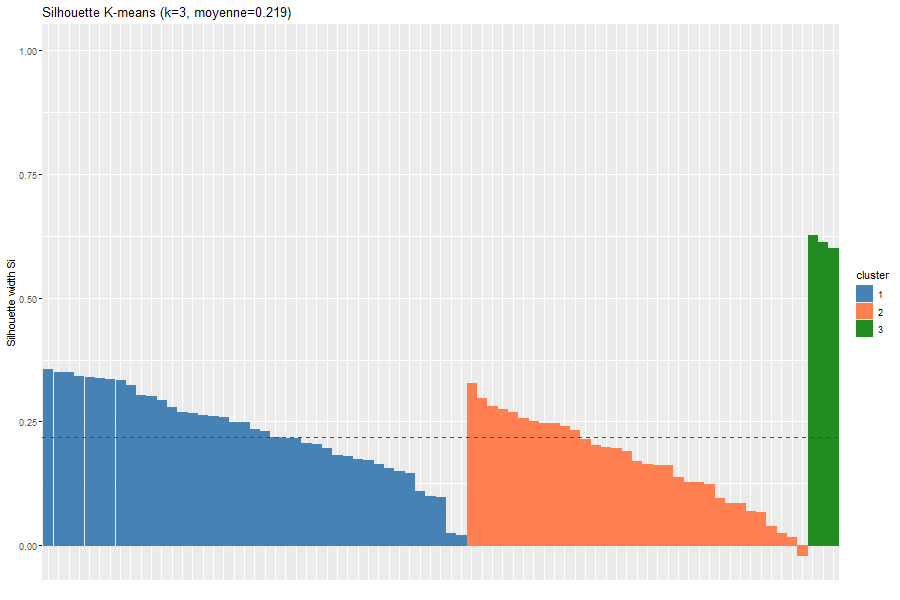
\includegraphics[width=0.6\linewidth]{output/figures/21_silhouette_kmeans} 

}

\caption{Silhouette des clusters K-means}\label{fig:silhouette}
\end{figure}

L'indice de Rand entre les deux partitions vaut 0.882, donc un bon
accord. La pureté est de 0.935 : 93.5\% des céréales tombent dans le
même groupe selon les deux méthodes. Les rares désaccords concernent des
céréales à la limite entre les groupes ``sucre'' et ``modéré'', ce qui
n'a rien d'étonnant puisque cette frontière est moins marquée que la
séparation avec le groupe haute fibre.

\begin{figure}[H]

{\centering 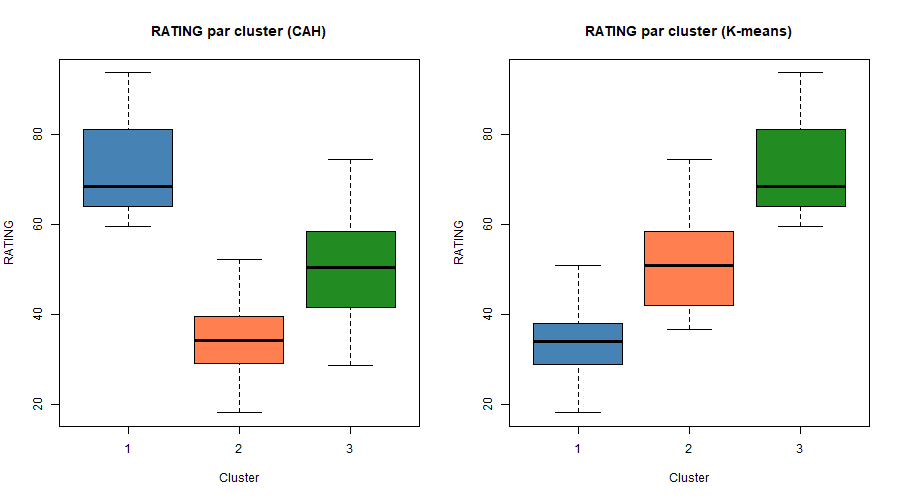
\includegraphics[width=0.65\linewidth]{output/figures/22_rating_par_cluster} 

}

\caption{RATING par cluster (K-means)}\label{fig:rating-clusters}
\end{figure}

Le RATING moyen par cluster va dans le même sens : 73.8 pour les
céréales haute fibre, 51.4 pour les modérées et 33.3 pour les sucrées.
La note de Consumer Reports pénalise le sucre et valorise les fibres, ce
qui correspond aux recommandations diététiques actuelles.

\section{Conclusion}\label{conclusion}

L'analyse du jeu ``276 céréales'' fait ressortir deux grands axes de
variation : d'un côté la teneur en fibres (et le potassium qui va avec),
de l'autre la densité calorique (calories, sucres, graisses). À eux
deux, ils expliquent plus de la moitié de la variance totale.

La classification en 3 groupes, retrouvée de façon cohérente par la CAH
et les K-means (Rand = 0.88), sépare un gros groupe de céréales
``sucrées/caloriques'', un groupe de céréales ``modérées/classiques'',
et un petit groupe très riche en fibres composé uniquement d'All-Bran.

Un point qui nous a marqués : RATING, qui n'entre pas dans le calcul des
axes, se projette presque parfaitement dans le plan factoriel. Elle est
liée positivement aux fibres et négativement aux sucres, ce qui laisse
penser que Consumer Reports juge la qualité nutritionnelle avec des
critères proches de ceux que sort l'ACP.

Il reste une limite : la partition en 3 clusters a une silhouette
moyenne faible (0.22) et le groupe haute fibre ne contient que 3
individus. Une partition en 2 clusters serait plus solide
statistiquement mais moins informative. Le choix de k=3 est un compromis
entre stabilité et finesse d'interprétation.

\section{Annexe : code R}\label{annexe-code-r}

Toute l'analyse tient dans un seul script,
\texttt{scripts/analyse\_cereales.R}, qui enchaîne le prétraitement, les
statistiques descriptives, l'ACP normée, la CAH, les K-means et la
synthèse. Il s'appuie sur les packages FactoMineR, factoextra, corrplot,
cluster et moments.

{\footnotesize
\begin{verbatim}
# Projet TND - Analyse des cereales
# ACP normee + CAH + K-means sur les 77 cereales de 276-cereals.txt
library(FactoMineR); library(factoextra); library(corrplot)
library(cluster); library(moments)
set.seed(42)

# --- Pretraitement ---------------------------------------------------------
cereales <- read.table("Binome5/276-cereals.txt", header = TRUE, sep = "\t",
                        strip.white = TRUE, quote = "", comment.char = "")
quanti <- c("CALORIES","PROTEIN","FAT","SODIUM","FIBER","CARBO","SUGARS",
            "POTASS","VITAMINS","SHELF","WEIGHT","CUPS","RATING")
for (c in quanti) {                       # -1 = donnee manquante
  cereales[[c]][cereales[[c]] == -1] <- NA
  cereales[[c]][is.na(cereales[[c]])] <- median(cereales[[c]], na.rm = TRUE)
}
cereales$MANUF <- factor(cereales$MANUF); cereales$TYPE <- factor(cereales$TYPE)
rownames(cereales) <- make.unique(trimws(cereales$NAME))
actives <- c("CALORIES","PROTEIN","FAT","SODIUM","FIBER","CARBO",
             "SUGARS","POTASS","VITAMINS")

# --- Statistiques descriptives ---------------------------------------------
print(round(data.frame(
  Moy = sapply(cereales[actives], mean), Med = sapply(cereales[actives], median),
  Sd  = sapply(cereales[actives], sd),  Skew = sapply(cereales[actives], skewness)), 2))
X <- scale(cereales[actives])
print(round(cor(cereales[actives]), 2))
corrplot(cor(cereales[actives]), method = "color", type = "upper",
         order = "hclust", addCoef.col = "black", tl.col = "black")

# --- ACP normee (variables suppl. : conditionnement, RATING, MANUF, TYPE) ---
acp <- PCA(cereales[, c(actives,"SHELF","WEIGHT","CUPS","RATING","MANUF","TYPE")],
           quanti.sup = 10:13, quali.sup = 14:15,
           scale.unit = TRUE, graph = FALSE)
print(round(acp$eig, 2))
print(round(acp$quanti.sup$coord[, 1:2], 2))   # projection de RATING
fviz_pca_var(acp, col.var = "contrib", repel = TRUE)
fviz_pca_biplot(acp, repel = TRUE, labelsize = 2)

# --- CAH (Ward, distance euclidienne) --------------------------------------
hc <- hclust(dist(X), method = "ward.D2")
for (k in 2:6)
  cat("k =", k, ": silhouette =",
      round(mean(silhouette(cutree(hc, k), dist(X))[, 3]), 3), "\n")
cereales$cah <- factor(cutree(hc, 3))
fviz_dend(hc, k = 3, rect = TRUE)

# --- K-means (k = 3, identique a la CAH) ------------------------------------
km <- kmeans(X, centers = 3, nstart = 25)
cereales$km <- factor(km$cluster)
prof <- aggregate(X, list(cereales$km), mean); rownames(prof) <- prof[, 1]
barplot(as.matrix(prof[, -1]), beside = TRUE, las = 2,
        col = c("steelblue","coral","forestgreen"))

# --- Comparaison des deux partitions ---------------------------------------
print(table(CAH = cereales$cah, Kmeans = cereales$km))
rand <- function(a, b) {                  # indice de Rand
  n <- length(a); s <- 0
  for (i in 1:(n-1)) for (j in (i+1):n)
    s <- s + ((a[i]==a[j]) == (b[i]==b[j]))
  s / choose(n, 2)
}
purete <- function(cl, ref)
  sum(tapply(ref, cl, function(x) max(table(x)))) / length(cl)
ca <- as.integer(cereales$cah); ke <- as.integer(cereales$km)
cat("Rand   :", round(rand(ca, ke), 3), "\n")
cat("Purete :", round(purete(ca, ke), 3), "\n")

# --- Synthese : clusters dans le plan ACP et lien avec RATING --------------
fviz_pca_ind(acp, habillage = cereales$km, addEllipses = TRUE,
             repel = TRUE, labelsize = 2)
print(round(tapply(cereales$RATING, cereales$km, mean), 1))
boxplot(RATING ~ km, data = cereales, col = c("steelblue","coral","forestgreen"))
\end{verbatim}
}

\end{document}
